\section{Технологический раздел}
В данном разделе выбраны средства реализации, в том числе определенный язык программирования и фреймворк, учитывая их поддержку работы с базами данных. Также была выбрана конкретная СУБД, представлены реализации создания баз данных, функции расчёта турнирной таблицы и ролевой модели. Кроме того, был представлен интерфейс приложения, предоставляющий возможность взаимодействия с базой данных, включая просмотр и редактирование данных.
\subsection{Средства реализации}
Для написания приложения был выбран язык программирования C\#, поскольку:
\begin{itemize}
    \item C\# объектно-ориентирован, что позволяет создавать классы, объекты и методы, упрощая моделирование объектов базы данных и их взаимосвязей;
    \item C\# имеет встроенный механизм LINQ \cite{linq}, который предоставляет объектно-ориентированный синтаксис для упрощения запросов к базе данных;
    \item C\# является частью .NET framework \cite{net}, который предоставляет широкий набор библиотек и инструментов для разработки приложений, работающими с базами данных.
\end{itemize}

В качестве среды разработки была выбрана Visual Studio, так как:
\begin{itemize}
    \item данная среда разработки является бесплатной;
    \item предоставляет удобный интерфейс для работы с Windows Forms \cite{forms} --- инструментом для создания графического интерфейса.
\end{itemize}

\subsection{Выбор СУБД}

В качестве СУБД была выбрана PostgreSQL. Данный выбор обусловлен следуюшими причинами:
\begin{itemize}
    \item PostgreSQL --- СУБД с открытым исходным кодом, что означает, что она свободно доступна для использования и модификации;
    \item данная СУБД обеспечивает детальный контроль доступа, позволяя определять роли пользователей, разрешения и ограничения доступа на различных уровнях;
    \item PostgreSQL позволяет расширять его функциональность с помощью пользовательских расширений и определяемых пользователем функций.
\end{itemize}

\subsection{Реализация создания таблиц базы данных}
В листинге \ref{lst:create1} представлено создание таблиц users, countries и tournaments.
\begin{lstlisting}[label=lst:create1,caption={Создание таблиц users, countries, tournaments}]
create table if not exists users
(
    id int not null primary key,
    login varchar(64) not null,
    password varchar(64) not null,
    permissions varchar(64) not null
);

create table if not exists countries
(
    id int not null primary key,
    name varchar(64) not null,
    confederation varchar(64) not null
);

create table if not exists tournaments
(
    id int not null primary key,
    name varchar(64) not null,
    country_id int,
    foreign key (country_id) references countries(id) on delete set null,
    user_id int not null,
    foreign key (user_id) references users(id) on delete cascade
);
\end{lstlisting}
В листинге \ref{lst:create2} представлено создание таблиц teams, matches и team\_tournaments.
\newpage
\begin{lstlisting}[label=lst:create2,caption={Создание таблиц teams, matches, team\_tournaments}]
create table if not exists teams
(
    id int not null primary key,
    name varchar(64) not null,
    country_id int,
    foreign key (country_id) references countries(id) on delete set null 
);

create table if not exists matches
(
    id int not null primary key,
    tournament_id int not null,
    foreign key (tournament_id) references tournaments(id) on delete cascade,
    home_team_id int not null,
    foreign key (home_team_id) references teams(id) on delete cascade,
    guest_team_id int not null,
    foreign key (guest_team_id) references teams(id) on delete cascade,
    home_goals int not null,
    guest_goals int not null
);

create table if not exists team_tournaments
(
    team_id int not null,
    foreign key (team_id) references teams(id) on delete cascade,
    tournament_id int not null,
    foreign key (tournament_id) references tournaments(id) on delete cascade,
    primary key(team_id, tournament_id)
);
\end{lstlisting}
\subsection{Реализация функции расчёта турнирной таблицы}
В листингах \ref{lst:func1} и \ref{lst:func2} представлена функция расчёта турнирной таблицы.
\newpage
\begin{lstlisting}[label=lst:func1,caption={Функция расчёта турнирной таблицы (часть 1)}]
create or replace function get_table(id_ integer)
returns table(name varchar(64), matches integer, wins integer, draws integer, loses integer, gs integer, gc integer, points integer)
as $$
begin
	drop table if exists tour_clubs;
	create temp table if not exists tour_clubs(id integer, name varchar(64));
    insert into tour_clubs(id, name)
	select c.id, c.name
	from teams c join team_tournaments tt on c.id = tt.team_id
		join tournaments t on tt.tournament_id = t.id
	where t.id = id_;

	drop table if exists home_results;
	create temp table if not exists home_results(id integer, matches integer, wins integer, draws integer, loses integer, gs integer, gc integer);
	insert into home_results(id, matches, wins, draws, loses, gs, gc)
	select c.id, count(*), sum(case when m.home_goals > m.guest_goals then 1 else 0 end),
		sum(case when m.home_goals = m.guest_goals then 1 else 0 end),
		sum(case when m.home_goals < m.guest_goals then 1 else 0 end),
		sum(m.home_goals), sum(m.guest_goals)

	from tour_clubs c join matches m on c.id = m.home_team_id
	where m.tournament_id = id_
	group by c.id;

	drop table if exists guest_results;
    create temp table if not exists guest_results(id integer, matches integer, wins integer, draws integer, loses integer, gs integer, gc integer);
	insert into guest_results(id, matches, wins, draws, loses, gs, gc)
	select c.id, count(*), 
		sum(case when m.home_goals < m.guest_goals then 1 else 0 end),
		sum(case when m.home_goals = m.guest_goals then 1 else 0 end),
		sum(case when m.home_goals > m.guest_goals then 1 else 0 end),
		sum(m.guest_goals), sum(m.home_goals)
\end{lstlisting}
\begin{lstlisting}[label=lst:func2,caption={Функция расчёта турнирной таблицы (часть 2)}]
	from tour_clubs c join matches m on c.id = m.guest_team_id
	where m.tournament_id = id_
	group by c.id;

	drop table if exists results;
    create temp table if not exists results(name varchar(64), matches integer, wins integer, draws integer, loses integer, gs integer, gc integer, diff integer, points integer);
	insert into results(name, matches, wins, draws, loses, gs, gc, diff, points)
	select c.name, h.matches + g.matches, h.wins + g.wins, h.draws + g.draws, h.loses + g.loses,
		h.gs + g.gs, h.gc + g.gc, 
		h.gs + g.gs - h.gc - g.gc,
		(h.wins + g.wins) * 3 + h.draws + g.draws
	from tour_clubs c join home_results h on c.id = h.id
		join guest_results g on c.id = g.id;
	return query
	select r.name, r.matches, r.wins, r.draws, r.loses, r.gs, r.gc, r.points
	from results r
	order by r.points desc, r.diff desc, r.wins desc;

end
$$ language PLPGSQL
\end{lstlisting}

\subsection{Реализация ролевой модели}
В листингах \ref{lst:role1} и \ref{lst:role2} представлены создание ролей и наделение их правами доступа.
\begin{lstlisting}[label=lst:role1,caption={Создание ролей и наделение их правами доступа (часть 1)}]
CREATE ROLE admin WITH
    CONNECTION LIMIT -1
    LOGIN
    PASSWORD 'admin';

GRANT ALL PRIVILEGES 
    ON ALL TABLES IN SCHEMA public 
    TO admin;
\end{lstlisting}

\begin{lstlisting}[label=lst:role2,caption={Создание ролей и наделение их правами доступа (часть 2)}]
CREATE ROLE _user WITH
    CONNECTION LIMIT -1
    LOGIN
    PASSWORD 'user';
    
GRANT SELECT
    ON ALL TABLES IN SCHEMA public 
    TO _user;

GRANT INSERT
    ON public."teams", 
       public."tournaments", 
       public."team_tournaments",
       public."matches"
    TO _user;

GRANT DELETE
    ON public."tournaments", 
       public."team_tournaments",
       public."matches"
    TO _user;

GRANT UPDATE
    ON public."matches"
    TO _user;

CREATE ROLE guest WITH
    CONNECTION LIMIT -1
    LOGIN
    PASSWORD 'guest';

GRANT SELECT
    ON ALL TABLES IN SCHEMA public 
    TO guest;

GRANT INSERT
    ON public."users"
    TO guest;
\end{lstlisting}

\subsection{Интерфейс приложения}
При запуске приложение открывается меню, продемонстрированное на рисунке \ref{img:menu}. При этом изначально пользователь является неавторизованным (гостем).
\begin{figure}
  \centering
  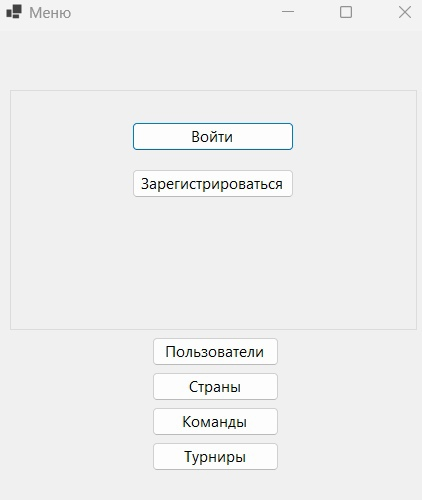
\includegraphics[scale=0.5]{inc/menu}
  \caption{Меню приложения}
  \label{img:menu}
\end{figure}
На рисунках \ref{img:login} и \ref{img:reg} представлены окно входа в аккаунт и окно регистрации соответственно.
\begin{figure}
  \centering
  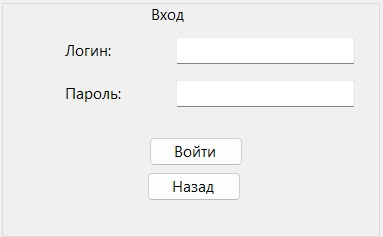
\includegraphics[scale=0.5]{inc/login.jpg}
  \caption{Окно входа}
  \label{img:login}
\end{figure}
\begin{figure}
  \centering
  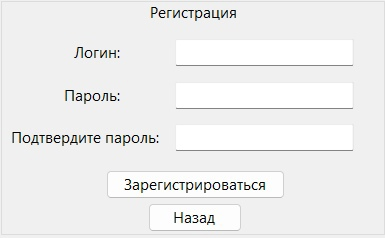
\includegraphics[scale=0.5]{inc/register.jpg}
  \caption{Окно регистрации}
  \label{img:reg}
\end{figure}
Далее окна будут показаны в том виде, в котором они открываются для администратора, для отображения всего функционала приложения.

На рисунке \ref{img:users} представлено окно просмотра пользователей.
\begin{figure}
  \centering
  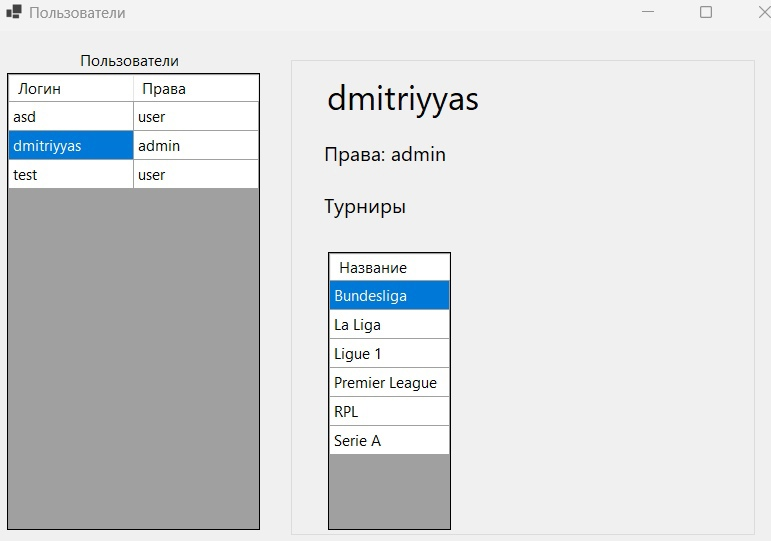
\includegraphics[scale=0.5]{inc/users.jpg}
  \caption{Окно просмотра пользователей}
  \label{img:users}
\end{figure}

На рисунке \ref{img:cou} представлено окно просмотра стран. В случае, если пользователь не обладает правами администратора, кнопка <<Создать страну>> не будет активна.
\begin{figure}
  \centering
  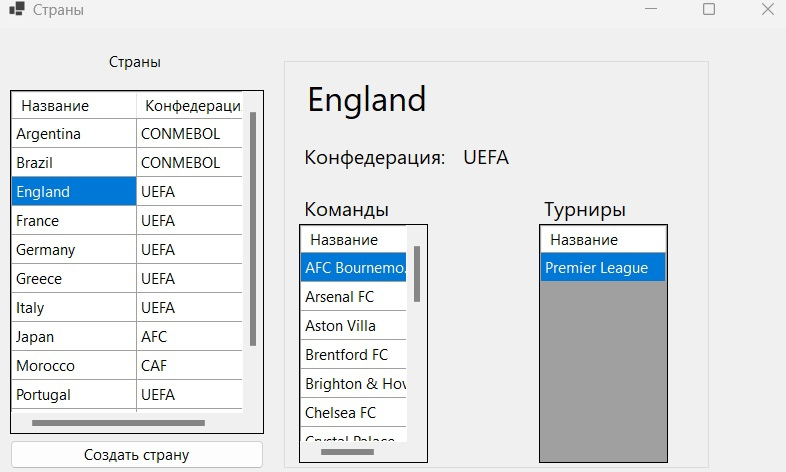
\includegraphics[scale=0.5]{inc/countries.jpg}
  \caption{Окно просмотра стран}
  \label{img:cou}
\end{figure}
На рисунке \ref{img:couc} представлено окно создания страны.
\begin{figure}
  \centering
  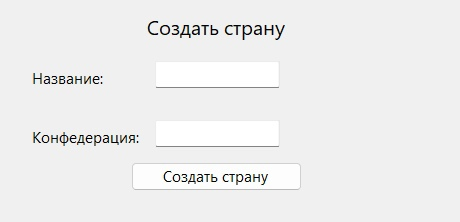
\includegraphics[scale=0.5]{inc/countrycr.jpg}
  \caption{Окно создания страны}
  \label{img:couc}
\end{figure}

На рисунке \ref{img:tea} представлено окно просмотра команд. В случае, если пользователь не авторизован, кнопка <<Создать команду>> не будет активна.
\begin{figure}
  \centering
  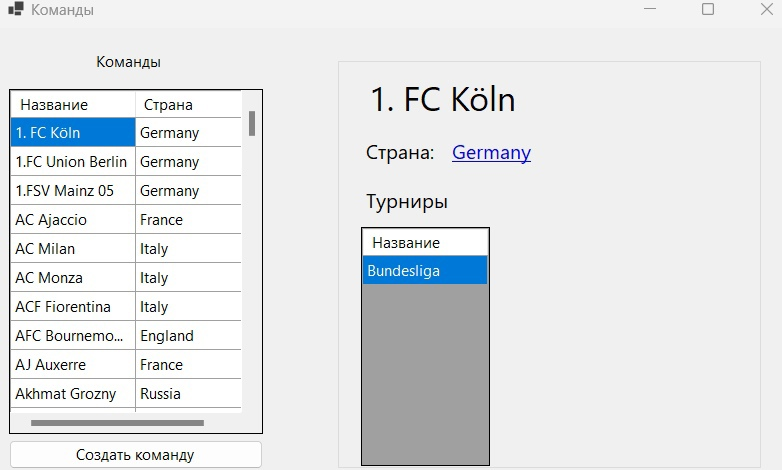
\includegraphics[scale=0.5]{inc/teams.jpg}
  \caption{Окно просмотра команд}
  \label{img:tea}
\end{figure}
На рисунке \ref{img:teac} представлено окно создания команды.
\begin{figure}
  \centering
  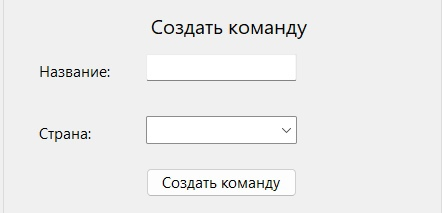
\includegraphics[scale=0.5]{inc/teamscr.jpg}
  \caption{Окно создания команды}
  \label{img:teac}
\end{figure}

На рисунке \ref{img:tou} представлено окно просмотра турниров. В случае, если пользователь не авторизован, кнопка <<Создать турнир>> не будет активна, а если пользователь просматривает чужой турнир, то кнопка <<Удалить турнир>> не будет активна.
\begin{figure}
  \centering
  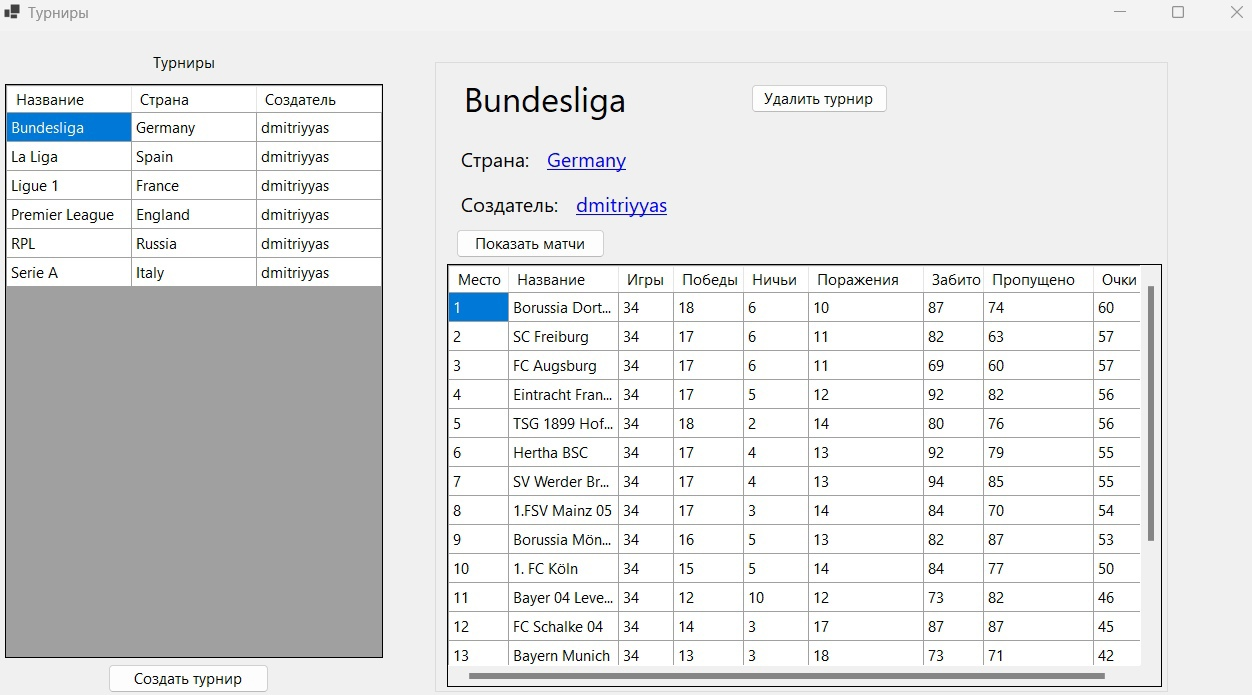
\includegraphics[scale=0.38]{inc/tours.jpg}
  \caption{Окно просмотра турниров}
  \label{img:tou}
\end{figure}
На рисунке \ref{img:touc} представлено окно создания турнира.
\begin{figure}
  \centering
  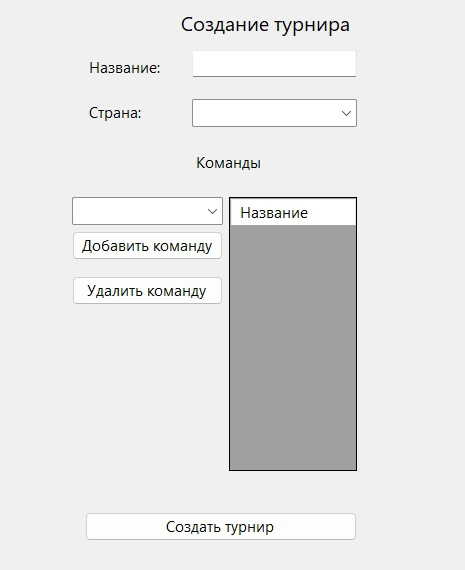
\includegraphics[scale=0.45]{inc/tourscr.jpg}
  \caption{Окно создания турнира}
  \label{img:touc}
\end{figure}
На рисунке \ref{img:tou2} представлено окно просмотра турниров после нажатия на кнопку <<Показать матчи>>.
\begin{figure}
  \centering
  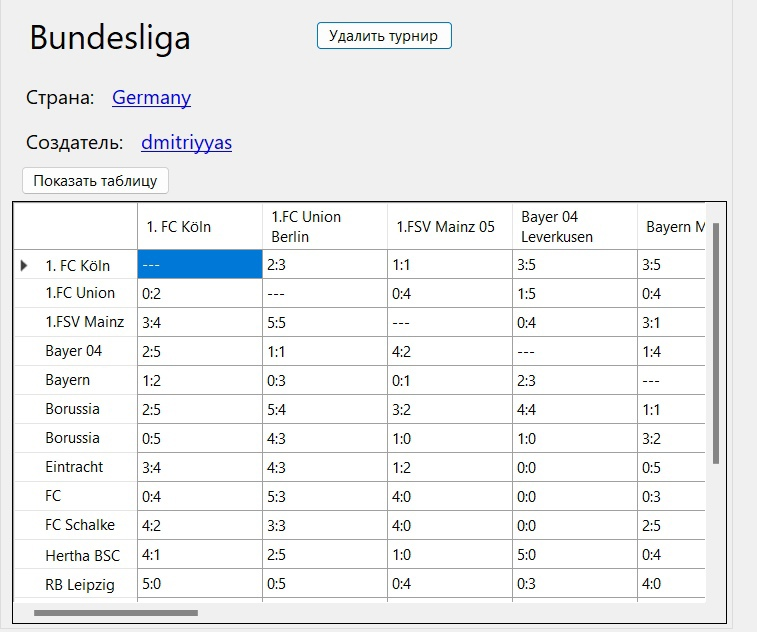
\includegraphics[scale=0.45]{inc/tours2.jpg}
  \caption{Окно просмотра матчей турнира}
  \label{img:tou2}
\end{figure}

На рисунке \ref{img:mat} представлено окно просмотра матча. В случае, если пользователь просматривает матч чужого турнира, кнопки <<Сохранить матч>> и <<Удалить матч>> не будут активны.
\begin{figure}
  \centering
  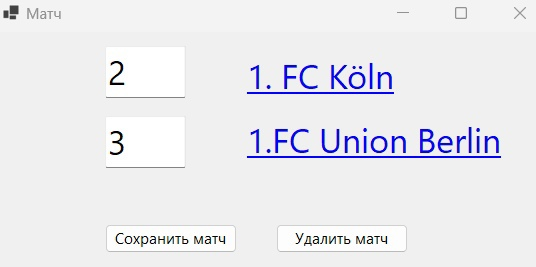
\includegraphics[scale=0.5]{inc/match.jpg}
  \caption{Окно просмотра матча}
  \label{img:mat}
\end{figure}

На рисунке \ref{img:matc} представлено окно создания матча. В случае, если пользователь просматривает матч чужого турнира, кнопка <<Создать матч>> не будет активна.
\begin{figure}
  \centering
  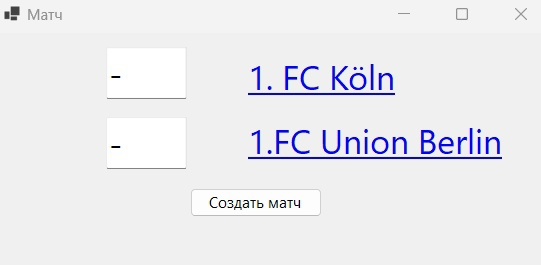
\includegraphics[scale=0.5]{inc/matchcr.jpg}
  \caption{Окно создания матча}
  \label{img:matc}
\end{figure}

\subsection*{Вывод}
В данном разделе были выбраны средства реализации --- язык программирования C\# и среда разработки Visual Studio. В качестве СУБД была выбрана PostgreSQL. Также был приведен интерфейс пользователя.